\newpage
\section*{Capítulo 8. Diseño del sistema}
\addcontentsline{toc}{section}{Capítulo 8. Diseño del sistema}
\setcounter{section}{8}
\setcounter{subsection}{0}

El diseño del sistema propone una arquitectura distribuida en tres componentes principales: la aplicación móvil, la plataforma web y la infraestructura en Amazon Web Services (AWS). 

\subsection{Arquitectura general del sistema}

Para garantizar su operatividad en entornos sin conexión, como el Bosque de Chapultepec, el cliente móvil emplea una estrategia \textit{offline-first}. La captura de imágenes y la inferencia para la detección de insectos se ejecutan localmente mediante TensorFlow Lite, sincronizando los datos hacia la nube de forma eventual y segura al recuperar la conectividad.

La arquitectura en la nube se basa en un enfoque \textit{serverless} mediante Amazon API Gateway y AWS Lambda, con autenticación gestionada por Amazon Cognito. El ciclo de vida del modelo de Deep Learning recae en Amazon SageMaker, utilizando Amazon S3 y RDS para la persistencia de datos. El cliente web distribuye su contenido a través de Amazon CloudFront. Finalmente, para asegurar un entorno de grado de producción, la arquitectura integra AWS Certificate Manager (ACM) para el cifrado SSL/TLS, GitHub Actions para despliegues continuos (CI/CD) y una capa transversal de monitoreo centralizado con Amazon CloudWatch.

\begin{figure}[H]
    \centering
    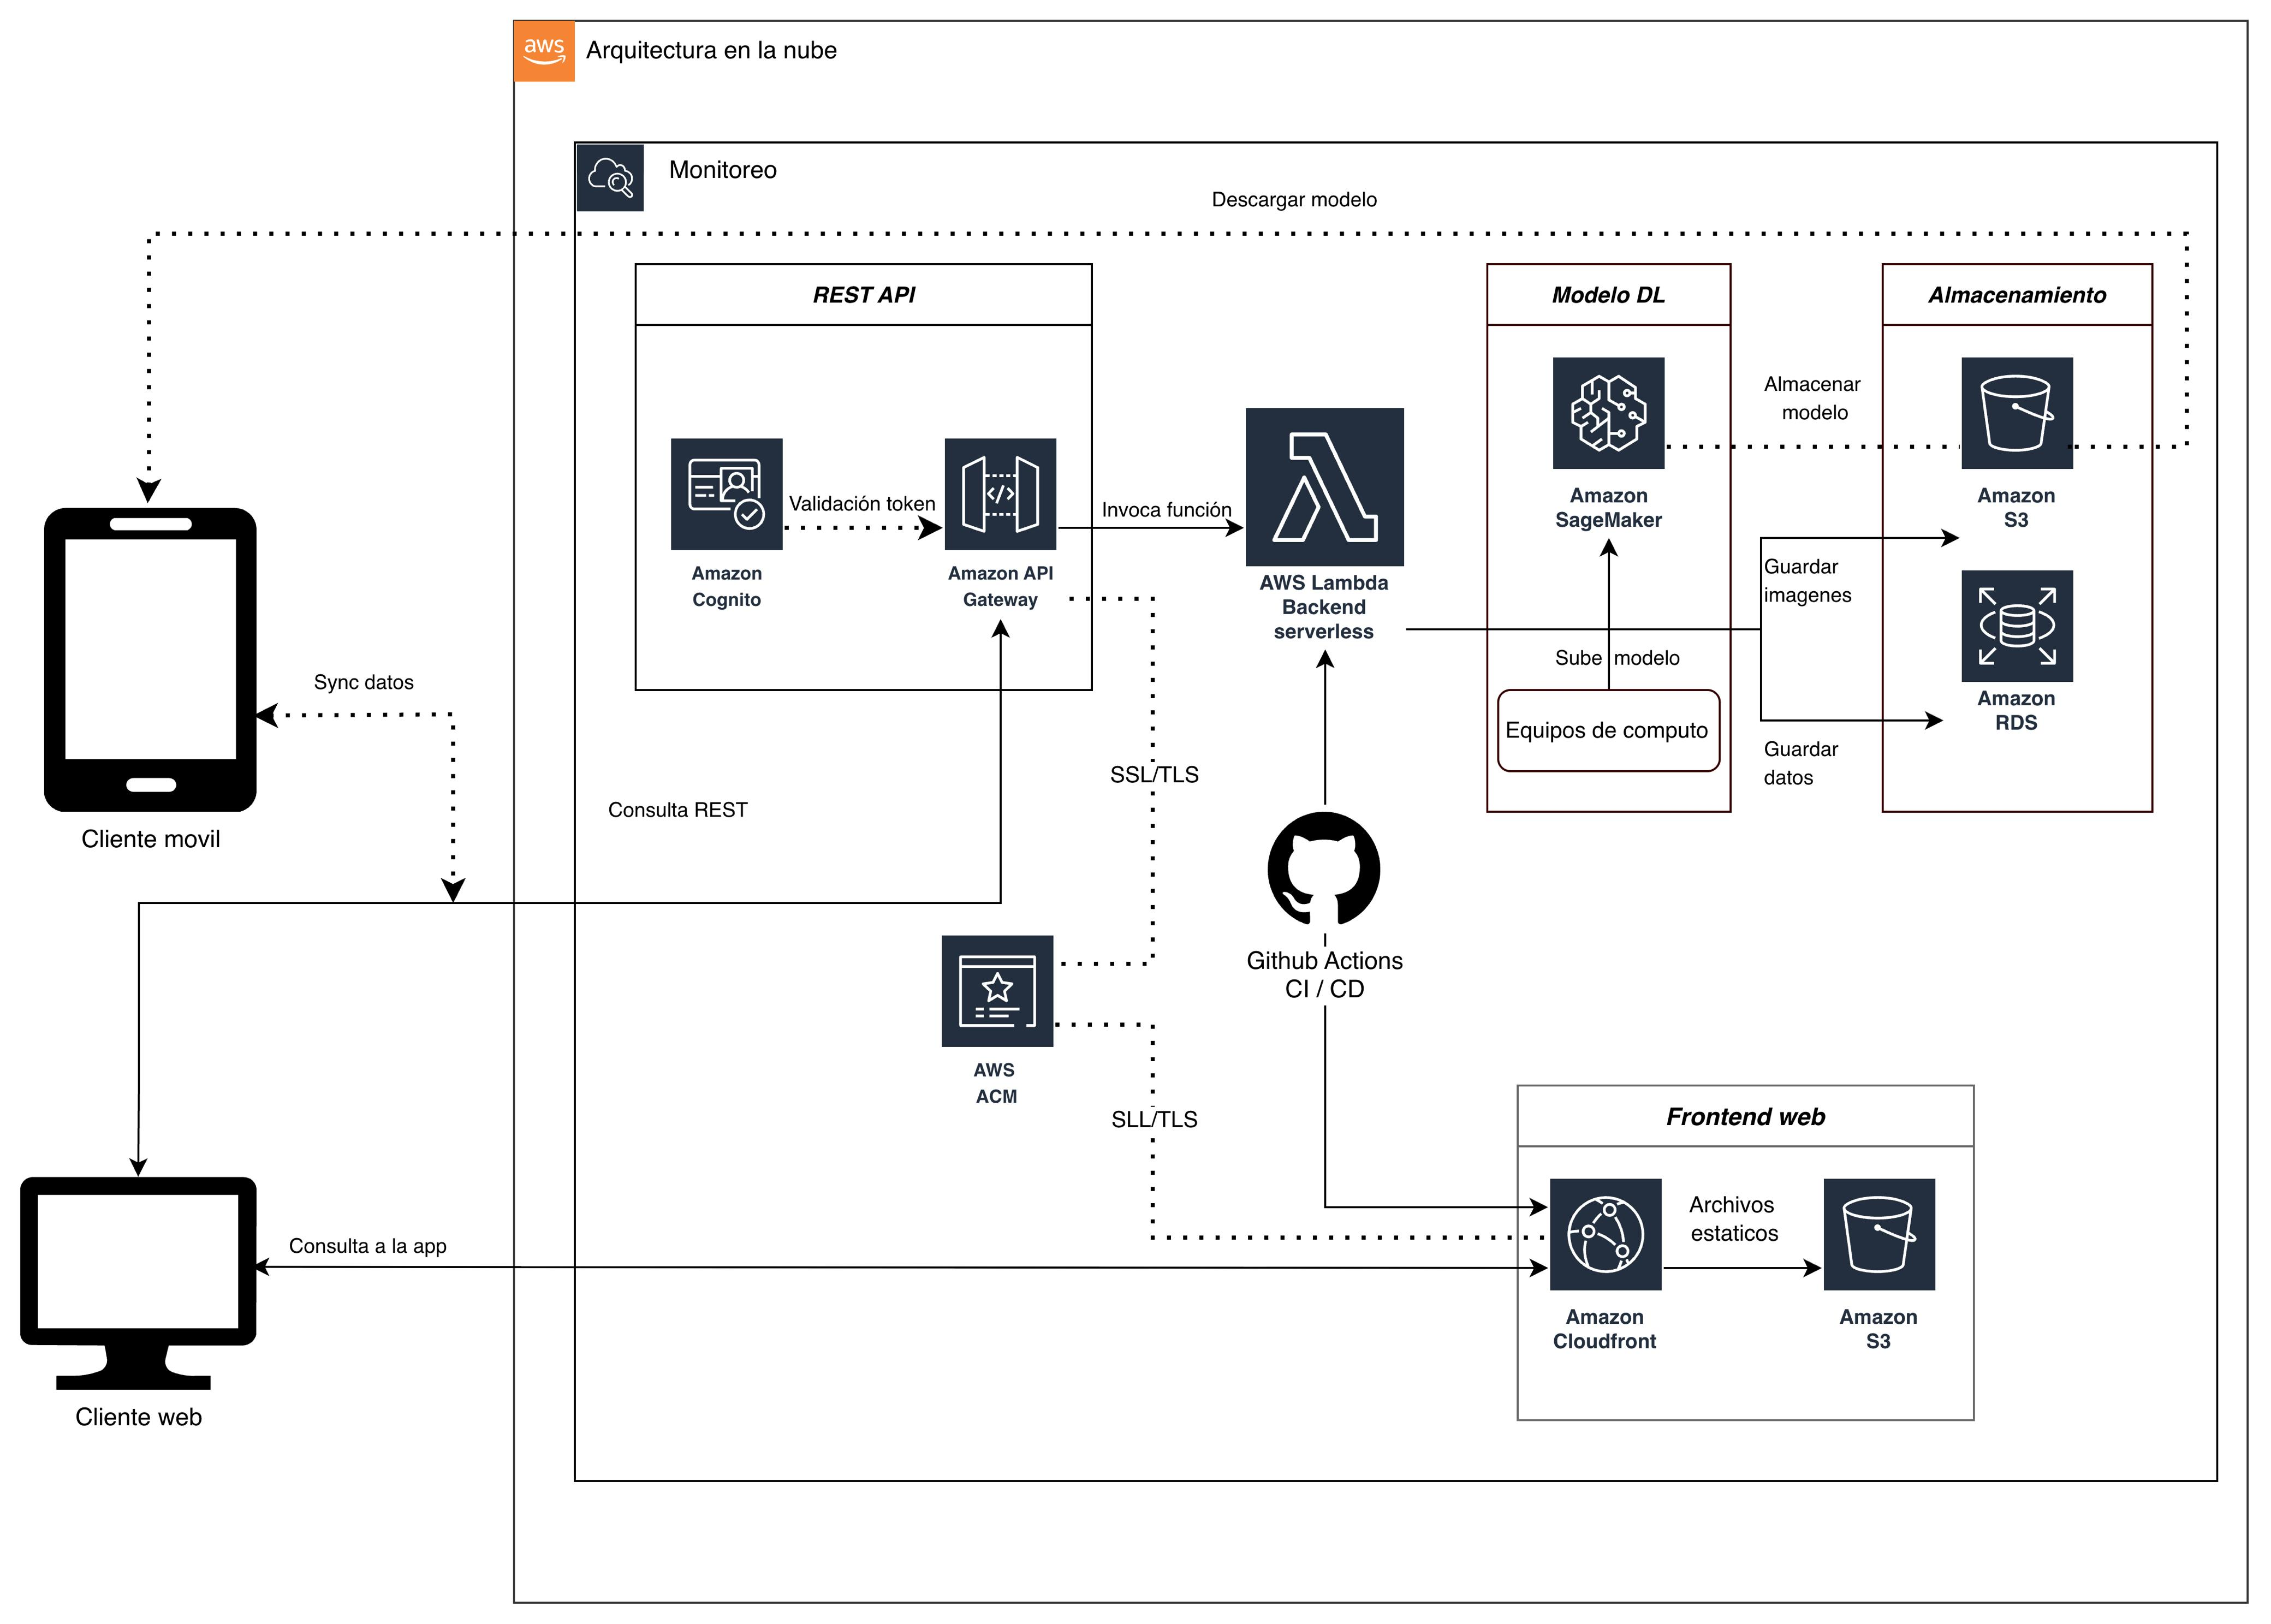
\includegraphics[width=0.95\textwidth]{images/C8/arquitectura_general.jpeg}
    \caption{Arquitectura general del sistema.}
    \label{fig:arquitectura-general}
\end{figure}